\documentclass{TheAlternativeCourse}

\usepackage{menukeys}
\usepackage{tabularx}
\usepackage{float}
\usepackage{caption}

\title{Console Toolkit Exercises}
\date{}
\author{}

\begin{document}
\maketitle

\setlength{\parindent}{0cm}
\setlength{\parskip}{12pt}

\section{Introduction}

Welcome to this exercise session! This is a practical exercise on the Linux
command line.  If you have any question about the exercises, feel free to ask
the helpers for assistance.

\subsection*{Difficulty}

The exercises are designed in such a way that you will have to find solutions
by reading the manuals and using search engines. You are expected to come up
with appropriate solutions on your own, there will be no step-by-step guided
exercises!

There will be quite simple exercises for complete beginners at the start,
but there are also some much more difficult ones further into the exercise.
Feel free to skip ahead!

\subsection*{Liability}

By taking part in this exercise, you acknowledge that you alone are responsible
for your computer. TheAlternative and its parent organisation, the Student
Sustainability Commission, will not be held liable for any damages or loss of
data.

\pagebreak

\section{Basics}

To solve some of the exercises, you will need to download some files. Whenever
you see an orange box like below, this means you have a task to solve.

\begin{exercisebox}{Getting the repository}
    Open a terminal and enter the following (all on one line): \\
    \texttt{curl https://files.project21.ch/LinuxDays-Public/HS18-exercise.zip
        -o exercise.zip} \\\\
    Then extract the zip archive like this: \\
    \texttt{unzip exercises.zip}
\end{exercisebox}

\subsection{Running a command}

To run a command, you just type it into the console and hit enter.  Most useful
commands require some arguments. Arguments are given after the name of the
command, separated by spaces. There are also so-called \emph{flags}, which set
some options to alter the behaviour of a command. They have the form
\texttt{-x} (single letter form) or \texttt{--long-option} (long format).

An example of a more involved command:

\begin{cmdbox}
\texttt{ls -l --human-readable \textasciitilde/Downloads}
\end{cmdbox}

\subsection{Getting help}

\texttt{man} is a command you will need throughout the following
exercises.  It stands for ``manual'' and shows you what almost any given
command can do and which options are available for it.  Almost all commands
provide such a ``manpage'', which is typically written by the developers
themselves.

\begin{exercisebox}{The manual's manual}
    The \texttt{man} command itself has its own manpage. Type \texttt{man man}
    to access it, use the arrow keys to scroll, and press \keys{q} to exit.
    Have a look around, especially at the different section numbers.
    What is the section number for system calls?
\end{exercisebox}

An alternative to using the man pages is to try and see if a command has a help
option. This is usually displayed by appending the option \texttt{--help} after
the name of the command, which will often display much shorter and concise
instructions
on how to use a command.

\begin{exercisebox}{The help option}
    Look at the help output of \texttt{ls}. What is the flag to see hidden
    files?
\end{exercisebox}

\subsection{Navigating directories}

You can navigate your file system in the terminal, just like you could with
a graphical program. Below are the most important commands.

\begin{table}[H]
    \centering
    \rowcolors{1}{lightblue}{white}
    \begin{tcolorbox}[%
        enhanced,
        width=1.0\linewidth,
        fuzzy shadow={1mm}{-1mm}{0mm}{0.1mm}{black!50!white},
        tabularx={>{\centering\arraybackslash}l|>{\centering\arraybackslash}X},
        title={Commands for navigating directories}]
        \textbf{Command} & \textbf{Description} \\
        \texttt{pwd} & Display the current working directory. \\
        \texttt{tree DIR} & Get a visualization of the directory tree under
	    \texttt{DIR}. \\
        \texttt{ls DIR} & List all files and directories in the current
            working directory. \\
        \texttt{cd DIR} & Change the current working directory to the given
            directory. \\
    \end{tcolorbox}%
    \label{tab1}
\end{table}

\begin{exercisebox}{Making yourself at home}
    Have a look around your home directory and try out the mentioned commands.
    You will most likely recognise the layout from your graphical file browser.
    Remember you can always return to your home directory by running
    \texttt{cd} without any arguments.
\end{exercisebox}

\subsection{Modifying directories}

Just like in graphical programs, you can create and delete directories on the
command line.

\begin{table}[H]
    \centering
    \rowcolors{1}{lightblue}{white}
    \begin{tcolorbox}[%
        enhanced,
        fuzzy shadow={1mm}{-1mm}{0mm}{0.1mm}{black!50!white},
        width=1.0\linewidth,
        tabularx={>{\centering\arraybackslash}l|>{\centering\arraybackslash}X},
        title={Commands for modifying directories}]
        \textbf{Command} & \textbf{Description} \\
        \texttt{mkdir DIR} & Create a new directory with the given name. \\
        \texttt{rmdir DIR} & Remove a directory. Will not work with
            non-empty directories. \\
        \texttt{rm -r DIR} &  Remove a directory and its contents.
            {\color{exclamred}Attention! There is no trashcan on the command
            line!  Files and directories will be deleted irrevocably.} \\
        \texttt{cp -r SOURCE TARGET} &  Copy a source directory
            (recursively with all its contents) to a target. \\
        \texttt{mv SOURCE TARGET} & Move a file or directory.
            Also used to rename files/directories. \\
    \end{tcolorbox}%
    \label{tab2}
\end{table}

\begin{exercisebox}{Creating your first directory}
    Create a directory for the following exercises (you can call it
    \texttt{console-toolkit}). Change into that directory and create a file
    called \texttt{notes}. Then move the exercise file directory you downloaded
    in task 2.1 into your newly created directory.
\end{exercisebox}

\subsection{Viewing files}
If you want to view the contents of a text file, you have the following
options:

\begin{table}[H]
    \centering
    \rowcolors{1}{lightblue}{white}
    \begin{tcolorbox}[%
        enhanced,
        fuzzy shadow={1mm}{-1mm}{0mm}{0.1mm}{black!50!white},
        width=1.0\linewidth,
        tabularx={>{\centering\arraybackslash}l|>{\centering\arraybackslash}X},
        title={Commands for viewing files}]
        \textbf{Command} & \textbf{Description} \\
        \texttt{cat FILE} & Output a file to the terminal. \\
        \texttt{head FILE} & Output the first couple of lines to the terminal. \\
        \texttt{tail FILE} & Output the last couple of lines to the terminal. \\
        \texttt{less FILE} & Browse a file in a visual viewer. \\
    \end{tcolorbox}%
    \label{tab3}
\end{table}

\begin{exercisebox}{Log files}
    \texttt{tail} is often used to inspect errors log files. Use tail to find the
    last three lines of \texttt{dmesg\_log} (in the exercise files).
\end{exercisebox}

\hintbox{\texttt{dmesg} is tool to view the log output of your kernel.}

\subsection{Console tips \& tricks}

There are many small things that can make your life when using the terminal
little bit easier.  Following is a table with the most important keyboard
shortcuts you can use to speed up your workflow.

\begin{table}[H]
    \centering
    \rowcolors{1}{lightblue}{white}
    \begin{tcolorbox}[%
        enhanced,
        fuzzy shadow={1mm}{-1mm}{0mm}{0.1mm}{black!50!white},
        width=1.0\linewidth,
        tabularx={>{\centering\arraybackslash}l|>{\centering\arraybackslash}X},
        title={Terminal keyboard shortcuts}]
        \keys{\ctrl}+\keys{w} & Delete one word backwards. \\
        \keys{\ctrl}+\keys{u} & Delete the entire line. \\
        \keys{\ctrl}+\keys{l} & Clear the terminal. \\
        \keys{\ctrl}+\keys{a} & Go to the beginning of the line. \\
        \keys{\ctrl}+\keys{e} & Go to the end of the line. \\
        \keys{\ctrl}+\keys{c} & Terminate the currently runnig process. \\
        \keys{\ctrl}+\keys{d} & Quit the shell. \\
    \end{tcolorbox}%
    \label{tab4}
\end{table}

\section{Files \& Permissions}

This section introduces you to basic commands related to files. We will first
look at a command that can be used for creating empty files.

The \texttt{touch} command is most frequently used for creating new, empty
files. If you check the manual, you will see that it can also change certain
file timestamps (access and modification times).

\begin{exercisebox}{The magic touch}
    Switch to your home directory. Execute \texttt{touch file}. A new file
    should have been created. Confirm that this is the case.
\end{exercisebox}
%
We already saw \texttt{cat} in the previous section. Another tool to look at
files is \texttt{less}. This command is great if you want to look at large
bodies of text because unlike \texttt{cat}, it has a built-in scroll function.
Once you are done looking at the file, you can quit with \keys{q}.

\subsection{Permissions}

We will now look at two commands to manage permissions.

\texttt{chown} stands for ``change owner''. It is used to change the owner of a
given file. It can also change the group ownership.

\begin{exercisebox}{Get off my lawn}
    Create a new, empty file (hint: \texttt{touch}) and use \texttt{chown} to
    change its ownership to the \texttt{root} user (you will probably need
    \texttt{sudo} for this). Try deleting it. Then change the ownership back to
    your own user.
\end{exercisebox}
%
A very similar command is \texttt{chmod}. \texttt{chmod} stands for ``change
file mode bits'' and controls the following permissions on any given file:

\begin{itemize}
    \setlength\itemsep{-9pt}
	\item Read: Who can see the file data.
	\item Write: Who can modify the file.
	\item Execute: Who is allowed to run the file (like a program or a script)
\end{itemize}

\hintbox{Permissions can be viewed using \texttt{ls -l}.}

\begin{exercisebox}{{Read, Write, Execute}}
    The read, write and execute permissions do different things, depending on
    whether they are set for directories or for files. Find out what they mean
    for files and directorues by playing around with the \texttt{chmod}
    command, readings its manual or searching on the internet.
\end{exercisebox}

\subsection{File tools}

There are a number of other commands that are frequently used to get
information on files:

\begin{table}[H]
    \centering
    \rowcolors{1}{lightblue}{white}
    \begin{tcolorbox}[%
        enhanced,
        fuzzy shadow={1mm}{-1mm}{0mm}{0.1mm}{black!50!white},
        width=1.0\linewidth,
        tabularx={>{\centering\arraybackslash}l|>{\centering\arraybackslash}X},
        title={Commands for getting information about files}]
        \textbf{Command} & \textbf{Description} \\
	    \texttt{wc \$file} & Display line, word, and character count of a file \\
        \texttt{diff \$file1 \$file2} & Show differences between files \\
	    \texttt{ln \$target \$link\_name} & Create a link \\
        \texttt{du \$file} & Estimate file space usage \\
        \texttt{df} & Report file system disk usage \\
    \end{tcolorbox}%
    \label{tab5}
\end{table}

In the next exercise we are going to read some text from the standard input
(also called \texttt{stdin}). Reading from \texttt{stdin} means you can just
type text into the console. When you are done, hit \keys{Enter} to enter a
newline and then hit \keys{\ctrl}+\keys{d}. This is the universal end-of-file
character in Unix-like systems. It signals to the command that it the input has
finished. You can even use this key shortcut to close your terminal.

\begin{exercisebox}{Cat tricks}
    Type the command \texttt{cat -}. This starts \texttt{cat} to read from
    \texttt{stdin}. Enter some text and observe what happens when you press
    \keys{Enter}. \texttt{cat} will just keep reading until the end-of-file
    character, so you can enter multiple lines of text. When you are done,
    terminate the input as described above.
\end{exercisebox}

\begin{exercisebox}{Counting words}
    Sometimes you might want to know the length of some text. First, consult
    \texttt{wc}'s manual to find out how you can read from standard input. Copy
    a line of text of your choice from the \texttt{wc} manual, then use the
    \texttt{wc} syntax that you looked up to read from standard input. Paste
    the text and terminate the input as before.
\end{exercisebox}

\hintbox{%
Copying and pasting in the console usually works with
\keys{\ctrl}+\keys{\shift}+\keys{c} and \keys{\ctrl}+\keys{\shift}+\keys{v},
this depends on the terminal though.}

\paragraph{Hardlink}
A hardlink is a pointer to a specific, physical location on a hard disk. If the
file name of the file that is linked to changes, the link still works. However,
if the file is replaced by a different file with the same name, the hardlink
will now \emph{not} point to the new file!  It will still point to the location
of the old file.

\paragraph{Symlink}
A symlink (short for symbolic link) points to a file name, to an actual file
path. If the data behind the file name is changed, the symbolic link will then
point to this new file, as long as the name stays the same. This is a higher
level concept than a hardlink, as it operates above the concept of file names.
Most of the time, a symlink is preferrable to a hardlink.

\begin{exercisebox}{Symlinks}
    Have a look at the \texttt{ln} manual to find out how to create a symbolic
    link. Then create a link in your home directory to a directory you use
    frequently.
\end{exercisebox}

Lastly, two commands that are loosely related to files are \texttt{df} and
\texttt{du}. These commands are used to find out how much space files take up.
\texttt{df} shows coarse-grained disk usage as reported by the file system.
\texttt{du} counts the disk usage of individual files and directories.

\begin{exercisebox}{Reporting disk usage}
    When you run \texttt{df} and \texttt{du}, the sizes of files are reported
    in multiples of blocks. The size of a block depends on your file system,
    but typically is between 512 bytes and 1 kilobyte. This means that you
    would have to multiply by this size the true size, in bytes. Find out how
    to make the output of \texttt{df} and \texttt{du} more readable for humans
    by looking at their options in the manual (hint: the option is the same for
    both tools).
\end{exercisebox}

\section{Leveraging the command line}

\subsection{Globbing (Wildcards)}

Globbing is a useful tool to work with files that share a pattern. For example,
to refer to all \texttt{jpg} images in a directory, you can use \texttt{*.jpg}.
The \texttt{*} means `any number of any characters', so this pattern will give
you all files that end with \texttt{.jpg}. Similarly, \texttt{dir/*} will give
you \emph{all} files in \texttt{dir}, \emph{except} hidden files.

There are a few more useful patterns, like \texttt{?} (question mark) which
matches any \emph{single} character, or \texttt{\string{*.jpg,*.png\string}},
which is a list that matches both \texttt{.jpg} and \texttt{.png} files. To
learn more, you can have a look at \texttt{man 7 glob}.

\begin{exercisebox}{{Printing text, again}}
    Ouput all \texttt{.txt} files in \texttt{notes/} to the terminal in
    a single command. The output will tell you if you did it correctly.
\end{exercisebox}

\begin{exercisebox}{Managing cat pictures}
    Create a new directory called \texttt{cats}. Copy all cat pictures in
    \texttt{pictures/} (in the exercise files) to your new \texttt{cats}
    directory, with a single command.
\end{exercisebox}

\subsection{Pipes}

Pipes are useful to connect multiple commands together. One of the design
principles of Unix was ``do one thing, and do it well''. This means, tools
should be simple and powerful in their specific domain, but there should also
be a mechanism to combine multiple programs in an easy way. This mechanism is
the \emph{pipe}, the \texttt{|} symbol. It allows you to connect the output of
one program to the input of another program.

For example, we can combine \texttt{du} and \texttt{sort} to work together.
\texttt{du} analyses the usage of disk space, and sort just sorts lines
it is given. This pipe analyzes your home directory and tells you which
directory uses the most space:

\begin{cmdbox}
    \texttt{du -sh * | sort -h}
\end{cmdbox}

Here the \texttt{*} globbing pattern stands for ``every file in the current
directory''.

\begin{exercisebox}{Counting lines in multiple files}
    \texttt{wc} (word count) can be used to count the number of lines in a file
    (\texttt{-l} flag). Use \texttt{cat} to output all files in the
    \texttt{notes} directory (exercise files) at the same time and connect it
    to \texttt{wc} to count the lines.
\end{exercisebox}

\subsection{Find}

Looking for specific files on your system is a task that one has to do fairly
regularly. Two very popular tool for finding files with certain properties are
\texttt{find} and \texttt{grep}. In this section, we cover \texttt{find}.  As a
rule of thumb, \texttt{find} is best used when you know that your file has
certain metadata: Maybe you know approximately when you have created the file,
when you last looked at it, how large it is etc. In contrast, \texttt{grep} is
usually used when you want to look at \emph{the content} of a file.

\texttt{find} works by essentially filtering all files through a chain of
conditions, given by flags. Working with \texttt{find} is
fairly straight forward and almost like verbally explaining what you are
looking for.

\begin{cmdbox}
find -mtime -1 -size +100k
\end{cmdbox}

This searches for all files that have been modified (\texttt{-mtime}) less than
one day ago (\texttt{-1}) and have size (\texttt{-size}) larger than 100
Kilobytes (\texttt{+100k}). \texttt{find} has a lot of conditions where it
makes sense to specify ``greater than'' or ``smaller than''. This is specified
by prefixing the amount with a \texttt{+} or a \texttt{-}. This is why the
condition ``larger than 100 Kilobytes'' is written as \texttt{-size +100k}.

If we additionally knew that our file was smaller than one gigabyte, we would
type:
\begin{cmdbox}
find -mtime -1 -size +100k -size -2G
\end{cmdbox}

It's necessary to use \texttt{-2G} here, since file sizes are rounded up.
A file that has 800M will be rounded to 1G. The semantics of find use strictly
smaller (\texttt{<}), therefore we have to compare to 2G.

Here is an overview of options for \texttt{find} that are useful to know.

\begin{table}[H]
    \centering
    \rowcolors{1}{lightblue}{white}
    \begin{tcolorbox}[%
        enhanced,
        fuzzy shadow={1mm}{-1mm}{0mm}{0.1mm}{black!50!white},
        width=1.0\linewidth,
        tabularx={>{\centering\arraybackslash}l|>{\centering\arraybackslash}X},
        title={Useful find flags}]
        \textbf{Flag} & \textbf{Description} \\
        \texttt{-name} & Matches the name of a file. \\
	    \texttt{-size} & Condition on the size of a file. \\
        \texttt{-atime} & Condition on when file was last accessed. \\
        \texttt{-mtime} & Condition on when file was last modified. \\
        \texttt{-type} & Specifies type of file (directory, regular file
        \ldots). \\
    \end{tcolorbox}%
    \label{tab6}
\end{table}

\begin{exercisebox}{The largest cat}
    Use \texttt{find} to find all cat pictures (\texttt{cat*}) with a size over
    200 kilobytes in the exercise directory. There should be more than one!
\end{exercisebox}

\subsection{Grep and regular expressions}

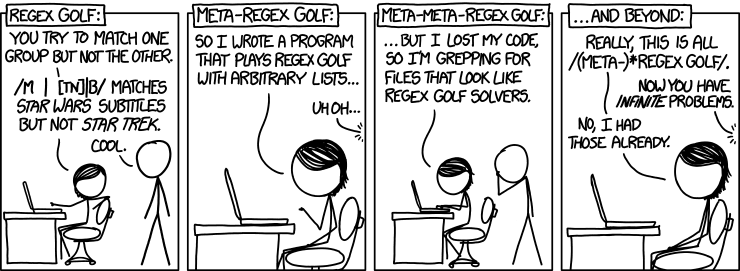
\includegraphics[width=\textwidth]{img/regex_golf.png}
{\footnotesize xkcd 1313, https://xkcd.com/1313/}

While working with many files in different folders, you can find yourself
losing track of what is in what file. To quickly find something in one of many
files, you can use \texttt{grep}. Grep is a tool for searching a body of text
for a specific pattern. Those patterns are specified with a syntax called
``Regular Expressions'' or regexes.

Regexes can easily become \emph{very} complicated (there are entire books on
this topic).  We'll have a look at the very basics here. Regexes are comprised
of a string of characters, e.g. \texttt{foo.bar[0-9]}. Let's look at it in more
detail:

\begin{itemize}
    \setlength\itemsep{-9pt}
    \item{\makebox[1.5cm]{\: \texttt{foo\hfill}} Matches the literal word ``foo''.}
    \item{\makebox[1.5cm]{\: \texttt{.\hfill}} Matches any single character.}
    \item{\makebox[1.5cm]{\: \texttt{bar\hfill}} Matches the literal word ``bar''.}
    \item{\makebox[1.5cm]{\: \texttt{[0-9]\hfill}} Matches a single digit between 0 and 9.}
\end{itemize}

For example, this regex \texttt{foo.bar[0-9]} would match on all of these
strings:

\begin{itemize}
    \setlength\itemsep{-9pt}
    \item \texttt{foo\_bar1}
    \item \texttt{fooobar9}
    \item \texttt{foozbar5}
    \item \texttt{foo1bar2}
\end{itemize}

An important thing to note is that regular expressions don't have to match the
entire string. So the example regex would also match on
\texttt{XXXXfoo1bar2XXXX}, because \texttt{foo1bar2} is part of that string.

So how do we try that on the command line? Simple, to test out \texttt{grep},
we can use \texttt{echo} to pipe a string into grep to match. Like this:

\begin{cmdbox}
    \texttt{echo foo1bar2 | grep foo.bar[0-9]}
\end{cmdbox}

This should output \texttt{foo1bar2}, because grep outputs all lines from its
input that match the regex.

There are a few command line options that you should know about \texttt{grep}.
These can also be combined, like so: \texttt{grep -rnoh PATTERN FILE}.

\begin{table}[H]
    \centering
    \rowcolors{1}{lightblue}{white}
    \begin{tcolorbox}[%
        enhanced,
        fuzzy shadow={1mm}{-1mm}{0mm}{0.1mm}{black!50!white},
        width=1.0\linewidth,
        tabularx={>{\centering\arraybackslash}l|>{\centering\arraybackslash}X},
        title={Useful grep flags}]
        \textbf{Command} & \textbf{Description} \\
        \texttt{-r} & Recursively look at all files under the given directory. \\
        \texttt{-o} & Only print the matching strings, not the entire line. \\
        \texttt{-h} & Don't print the filename, just the matching string/line. \\
        \texttt{-n} & Prefix the output with the linenumber where the match occured. \\
    \end{tcolorbox}%
    \label{tabgrepopts}
\end{table}

\begin{table}[H]
    \centering
    \rowcolors{1}{lightblue}{white}
    \begin{tcolorbox}[%
        enhanced,
        fuzzy shadow={1mm}{-1mm}{0mm}{0.1mm}{black!50!white},
        width=1.0\linewidth,
        tabularx={>{\centering\arraybackslash}l|>{\centering\arraybackslash}l|>{\centering\arraybackslash}X},
        title={Regex building blocks}]
        \textbf{Regex} & \textbf{Example} & \textbf{Description} \\

		\textbf{Match Expressions} & & \\
        \texttt{<character literal>} & \texttt{f} &
            Matches the character \texttt{<character literal>}.
            The example matches on \texttt{f}. \\
        \texttt{.} & \texttt{.} & Matches any single character. \\
        \texttt{[<char1>-<char2>]} & \texttt{[a-z]} &
            Matches a single character in the range from \texttt{<char1>} to
            \texttt{<char2>} (inclusive). The example matches on any lowercase
            character. The character range can be specified multiple times,
            like so: \texttt{[a-zA-Z0-9]}. This would match any lower- or
            uppercase character or digit. \\
        \texttt{[[:alnum:]]} & \texttt{[[:alnum:]]} &
            Alphanumeric characters (letters and digits). \\
        \texttt{[[:alpha:]]} & \texttt{[[:alpha:]]} & Letters. \\
        \texttt{[[:digit:]]} & \texttt{[[:digit:]]} & Digits. \\
        \texttt{[[:xdigit:]]} & \texttt{[[:xdigit:]]} & Hexadecimal digits. \\
        \texttt{[[:blank:]]} & \texttt{[[:blank:]]} & Blank space (spaces and tabs). \\
        \texttt{[[:word:]]} & \texttt{[[:word:]]} & Digits, letters and underscores. \\

		\textbf{Modifiers} & & \\
        \texttt{?} & \texttt{.?} &
            The preceding expression appears zero times or exactly once. The
            example would match on an empty string or any string of length one. \\
        \texttt{*} & \texttt{.*} &
            The preceding expression appears zero, one or many times. The
            example would match on a string of arbitrary length, including an
            empty one.\\
        \texttt{+} & \texttt{.+} &
            The preceding expression appears one or many times. The example
            matches on a string of any length greater than zero. \\
        \texttt{\string{<num>\string}} & \texttt{\string{3\string}} &
            Matches on a string if the preceding expression appears exactly
            \texttt{<num>} times. \\
        \texttt{\string{<num1>,<num2>\string}} & \texttt{\string{3,6\string}} &
            Matches on a string if the preceding expression appears between
            \texttt{<num1>} and \texttt{<num2>} times (inclusive). \\
    \end{tcolorbox}%
    \label{tabgreplarge}
\end{table}

\paragraph{Note} When using the characters \texttt{|, +, ?} with their regex
meaning, they must be escaped with a backslash like this: \verb@\|, \+, \?@. If
you want to use any of the ofter special characters as regular characters, i.e.
to match a literal \texttt{.} you can use \verb@\.@

\begin{exercisebox}{Finding email addresses}
    Somewhere in the exercise files, there is an email address hidden in a text
    file. Create a regular expression that matches email addresses that end in
    .ch and find it!
\end{exercisebox}

\section{Remote machines}

This section will be about working with remote machines. You will
connect to one and move files from and to it. Additionally, you will set up
your SSH so you can log in without entering a password.

\texttt{ssh} (secure shell) is an extremely useful tool, as it allows you to
manage servers, connecting to your home computer from a laptop, running
computations on super computers, and even using graphical applications that are
installed on a different computer. \texttt{scp} (secure copy) works just like
\texttt{cp}, but allows you to copy files to and from remote machines.
\texttt{scp} is based on the SSH protocol, so it works similiarly and the
public key authentication in exercise 5.2 will automatically also apply to
\texttt{scp}.

\begin{table}[H]
    \centering
    \rowcolors{1}{lightblue}{white}
    \begin{tcolorbox}[%
        enhanced,
        fuzzy shadow={1mm}{-1mm}{0mm}{0.1mm}{black!50!white},
        width=1.0\linewidth,
        tabularx={>{\centering\arraybackslash}l|>{\centering\arraybackslash}X},
        title={Remote access tools}]
        \texttt{ssh user@hostname} &
            Open an SSH session with a specific user on a host. \\
        \texttt{scp user@hostname:file.txt .} &
            Copy a file from remote machine to the current directory. \\
        \texttt{scp file.txt user@hostname:file.txt} &
            Copy a file from current directory to remote host. \\
    \end{tcolorbox}%
    \label{tab7}
\end{table}

\hintbox{%
If you don't have an ETH account, use\\
\texttt{hackingsession@pterodactyl.vsos.ethz.ch} with password\\
\texttt{BoredHacker} for the following exercises instead.}

\begin{exercisebox}{Establishing an SSH connection}
    Use SSH to connect to the Euler supercomputer at
    \texttt{nethz-login@euler.ethz.ch}, where \texttt{nethz-login} is your
    \emph{nethz} account name. You can login using your regular credentials.
\end{exercisebox}
%
It is inconvenient that you have to enter your password every time you want to
log in. You can set up SSH in a way where you \emph{don't} have to provide your
password!  This is done with public key cryptography. Basically, you generate a
public key and a private key.  The private key you keep safe and only for
yourself. The public key you can distribute to anyone.  Now you can
authenticate yourself for anyone that has your public key: You can create a
signature with your private key, that can be verified using the public key.
However, only the owner of the private key can create the signature that is
verifiable by the public key! This can be used by an SSH server to authenticate
clients that want to open an SSH session.

\begin{exercisebox}{Generating your key}
    Generate your private/public key pair using \texttt{ssh-keygen}.
    Then copy your generated public key (\texttt{.ssh/id\_rsa.pub}) to
    \texttt{.ssh/authorized\_keys} on the server. Try logging in with SSH now,
    it should no longer require a password.
\end{exercisebox}


\section{Jobs \& Processes}

Jobs are groups of processes that are running in the current shell. Often, a
job only consists of one process but sometimes a job is a process
\emph{pipeline} consisting of multiple jobs, such as
\texttt{echo "Hello" | cat -}. Consult the \texttt{JOB CONTROL} section
of the \texttt{bash} manual if you want to study the details.

Knowing how to control jobs is essential if you want to be able to
simultaneously run multiple processes from the same shell.

\subsection{Job control}

Jobs can be put into the background, started in the background, brought to the
foreground and killed. We say a job is running in the background when it is
currently running, but not blocking the shell. In other words, when a job is
running in the background, you can still use your shell normally (although the
job might produce output that will get displayed on your terminal which can be
quite annoying).

\begin{table}[H]
    \centering
    \rowcolors{1}{lightblue}{white}
    \begin{tcolorbox}[%
        enhanced,
        fuzzy shadow={1mm}{-1mm}{0mm}{0.1mm}{black!50!white},
        width=1.0\linewidth,
        tabularx={>{\centering\arraybackslash}l|>{\centering\arraybackslash}X},
        title={Working with jobs}]
	    \texttt{jobs} & List all jobs in the current shell\\
	    \texttt{cmd \&} & Start \texttt{cmd} in the background\\
	    \texttt{fg} & Bring a job into the foreground\\
	    \texttt{bg} & Bring a job into the background\\
    \end{tcolorbox}
    \label{tabjobcmds}
\end{table}

\begin{table}[H]
    \centering
    \rowcolors{1}{lightblue}{white}
    \begin{tcolorbox}[%
        enhanced,
        fuzzy shadow={1mm}{-1mm}{0mm}{0.1mm}{black!50!white},
        width=1.0\linewidth,
        tabularx={>{\centering\arraybackslash}l|>{\centering\arraybackslash}X},
        title={Controlling jobs}]
		\texttt{\keys{\ctrl}+\keys{z}} & Suspend current job. Processes may ignore this.\\
		\texttt{\keys{\ctrl}+\keys{c}} & Kill current job. Processes may ignore this.\\
        \texttt{kill N} & Kill job, where N is its number as listed in
        \texttt{jobs}.Processes may \emph{still} ignore this.\\
	    \texttt{kill -9 N} & Kill job with number N for sure.\\
    \end{tcolorbox}
    \label{tab8}
\end{table}

You can \emph{usually} use \keys{\ctrl}+\keys{c} to terminate a job in the
foreground and \keys{\ctrl}+\keys{z} to suspend a job in the foreground.
Suspended jobs are paused until they are resumed with either \texttt{fg} or
\texttt{bg}. Note that processes can choose to overwrite these shortcuts so
they are not guaranteed to work. If they don't work, we can always use more
drastic measures \ldots

\subsection{Processes}

Processes operate system-wide. Each process has a unique process ID, called the
PID for short. You can think of processes as separate programs running
independent of each other. For example, an \texttt{echo} command spawns a new
process that is separated from the shell process that you are in (which is
typically \texttt{bash}).

\begin{table}[H]
    \centering
    \rowcolors{1}{lightblue}{white}
    \begin{tcolorbox}[%
        enhanced,
        fuzzy shadow={1mm}{-1mm}{0mm}{0.1mm}{black!50!white},
        width=1.0\linewidth,
        tabularx={>{\centering\arraybackslash}l|>{\centering\arraybackslash}X},
        title={Managing}]
        \texttt{top} & Display info about all currently running processes. Quit
        with \keys{q}\\
        \texttt{htop} & A more modern equivalent of \texttt{top}. It is not
        installed by default on most distributions, but can be installed it
        with your package manager. \\
        \texttt{kill \texttt{PID}} & Send a termination signal to the process
        \texttt{PID}. This is the preferred way to terminate a process, as it
        allows it to exit normally and perform clean up. \\
        \texttt{kill -9 \texttt{PID}} & Send a killing signal to the
        process \texttt{PID}. The process is killed by the operating system
        immediately. Useful for unresponsive processes. \\
        \texttt{pkill \texttt{PATTERN}} & Like \texttt{kill}, but kills
        processes whose names match a pattern instead. \\
	    \texttt{pkill -9 \texttt{PATTERN}} & Send a kill signal instead. \\
        \texttt{ps} & Utility to display information about processes. Most
        commonly used as \texttt{ps aux}. \\
    \end{tcolorbox}%
    \label{tab9}
\end{table}

\texttt{kill} and \texttt{pkill} actually send so-called signals to processes.
There are many signals that all do different things. When you call \texttt{kill
PID}, the signal \texttt{15} is sent to the process \texttt{PID}. This signal
is called the \texttt{SIGTERM} signal and is used to \emph{ask} a process to
terminate. When we write \texttt{kill -9 PID}, we are actually sending the
signal \texttt{9} which is also known as \texttt{SIGKILL} and kills a process
instantly. Read \texttt{man 7 signal} if you want to know more about signals.


\begin{exercisebox}{Killed in their sleep}
    Start a new process by typing \texttt{sleep 1000} in your shell. Open
    another shell. Use \texttt{top}, \texttt{htop} or \texttt{ps} to figure out
    the PID of the \texttt{sleep} process. Kill it.
\end{exercisebox}

\begin{exercisebox}{A job for kill}
    \texttt{kill} also works on jobs. Start \texttt{sleep 1000} in the
    background (or start it in the foreground, suspend it, then bring it to the
    background). Then type \texttt{kill N} where \texttt{N} is the job's number
    (probably \texttt{1}). Check the output of the \texttt{jobs} command and
    confirm that the job is not displayed anymore.
\end{exercisebox}

\section{License}

This work is licensed under a Creative Commons Attribution-ShareAlike 4.0
International License. See also:
\url{http://creativecommons.org/licenses/by-sa/4.0/}.

\vspace{0cm}

\includegraphics[width=3cm]{assets/CC-BY-SA_icon.pdf}

\end{document}
